%%%% Better Poster latex template example v1.0 (2019/04/04)
%%%% GNU General Public License v3.0
%%%% Rafael Bailo
%%%% https://github.com/rafaelbailo/betterposter-latex-template
%%%% 
%%%% Original design from Mike Morrison
%%%% https://twitter.com/mikemorrison

\documentclass[a0paper,fleqn]{betterposter}

\usepackage{setspace}
\usepackage{multicol}
\usepackage{xcolor}
\usepackage{hyperref}

%%%% Uncomment the following commands to customise the format

%% Setting the width of columns
% Left column
\setlength{\leftbarwidth}{0.27\paperwidth}
% Right column
\setlength{\rightbarwidth}{0.27\paperwidth}

%% Setting the column margins
% Horizontal margin
%\setlength{\columnmarginvertical}{0.05\paperheight}
% Vertical margin
%\setlength{\columnmarginhorizontal}{0.05\paperheight}
% Horizontal margin for the main column
%\setlength{\maincolumnmarginvertical}{0.15\paperheight}
% Vertical margin for the main column
%\setlength{\maincolumnmarginhorizontal}{0.15\paperheight}

%% Changing font sizes
% Text font
%\renewcommand{\fontsizestandard}{\fontsize{28}{35} \selectfont}
% Main column font
%\renewcommand{\fontsizemain}{\fontsize{28}{35} \selectfont}
% Title font
%\renewcommand{\fontsizetitle}{\fontsize{28}{35} \selectfont}
% Author font
%\renewcommand{\fontsizeauthor}{\fontsize{28}{35} \selectfont}
% Section font
%\renewcommand{\fontsizesection}{\fontsize{28}{35} \selectfont}

%% Changing font sizes for a specific text segment
% Place the text inside brackets:
% {\fontsize{28}{35} \selectfont Your text goes here}
\renewcommand{\fontsizetitle}{\fontsize{72}{120} \selectfont}

\newcommand{\fontsizeinstitution}{\fontsize{26}{30} \selectfont}
\newcommand{\fontsizelarge}{\fontsize{40}{48} \selectfont}

\newcommand{\bigtext}[1]{{\fontsize{52pt}{56pt}\selectfont #1}}

\newcommand\orangefbox{\fcolorbox{orange}{white}}
\newcommand\purplefbox{\fcolorbox{purple}{white}}
\newcommand\redfbox{\fcolorbox{red}{white}}

%% Changing colours
% Background of side columns
%\renewcommand{\columnbackgroundcolor}{black}
% Font of side columns
%\renewcommand{\columnfontcolor}{gray}
% Background of main column
\renewcommand{\maincolumnbackgroundcolor}{empirical}
%\renewcommand{\maincolumnbackgroundcolor}{theory}
%\renewcommand{\maincolumnbackgroundcolor}{methods}
%\renewcommand{\maincolumnbackgroundcolor}{intervention}
% Font of main column
%\renewcommand{\maincolumnfontcolor}{black}
\renewcommand{\sectioncolor}{empirical}

%\definecolor{lightgreen}{RGB}{144,238,144}
\definecolor{lightgreen}{RGB}{83,166,83}
\definecolor{lightorange}{RGB}{255,166,0}
\definecolor{lightred}{RGB}{224,91,88}

\usepackage{fontspec}
\setmainfont[Scale=MatchLowercase]{FreeSerif}
\setmonofont[Scale=MatchLowercase]{DejaVu Sans Mono}

\newcommand\BibTeX{B{\sc ib}\TeX}

\newcommand{\archi}[1]{\texttt{{\color{lightgray}\{}#1{\color{lightgray}\}}}}
\newcommand{\mtag}[1]{\texttt{{\color{lightgray}<}#1{\color{lightgray}>}}}

\begin{document}	
\betterposter{
%%%%%%%% MAIN COLUMN

\maincolumn{
%%%% Main space
%The first ever published \textbf{morphological} analyser and generator for \textbf{Sakha}
\centering
The first ever published\\ \textbf{morphological}\\ \textbf{analyser \& generator}\\for \textbf{Sakha}
}{
%%%% Bottom space

%% QR code
%Change the code
\newqrcode{img/qrcode}{img/smartphoneWhite}{
%\textbf{Take a picture}
\textbf{Scan with mobile camera}
\\to access the code
\\\& download the poster
%\\for source, poster, and abstract
}{
\fontsizelarge{https://github.com/apertium/apertium-sah}}
% Smartphone icon
% Author: Freepik
% Retrieved from: https://www.flaticon.com/free-icon/smartphone_65680

%% Compact QR code (comment the previous command and uncomment this one to switch)
%\compactqrcode{img/qrcode}{
%\textbf{Take a picture} to
%\\download the full paper
%}

}

}{
%%%%%%%% LEFT COLUMN

\title{A Free/Open-Source\\ Morphological Analyser\\ and Generator for Sakha\\}
%\author{Sardana Ivanova \(\cdot\) \fontsizeinstitution{Helsingin yliopisto}}
%\author{Francis M. Tyers \(\cdot\) Indiana University}
%\author{Jonathan N. Washington \(\cdot\) Swarthmore College}
%\institution{Optional Institution Under Name}
\authorblock{0.3\textwidth}{Sardana Ivanova}{Helsingin yliopisto}~~~\authorblock{0.33\textwidth}{Jonathan N. Washington}{Swarthmore College}~~~\authorblock{0.3\textwidth}{Francis M. Tyers}{Indiana University}


\section{Background}
\textbf{Sakha} (\texttt{sah})
\begin{itemize}
\item Indigenous language of \textbf{Siberia}, official in Sakha Republic
\item \textbf{Turkic} language: agglutinating, vowel harmony
\item \textasciitilde{}0.5M speakers, under pressure from Russian
\end{itemize}
\begin{center}
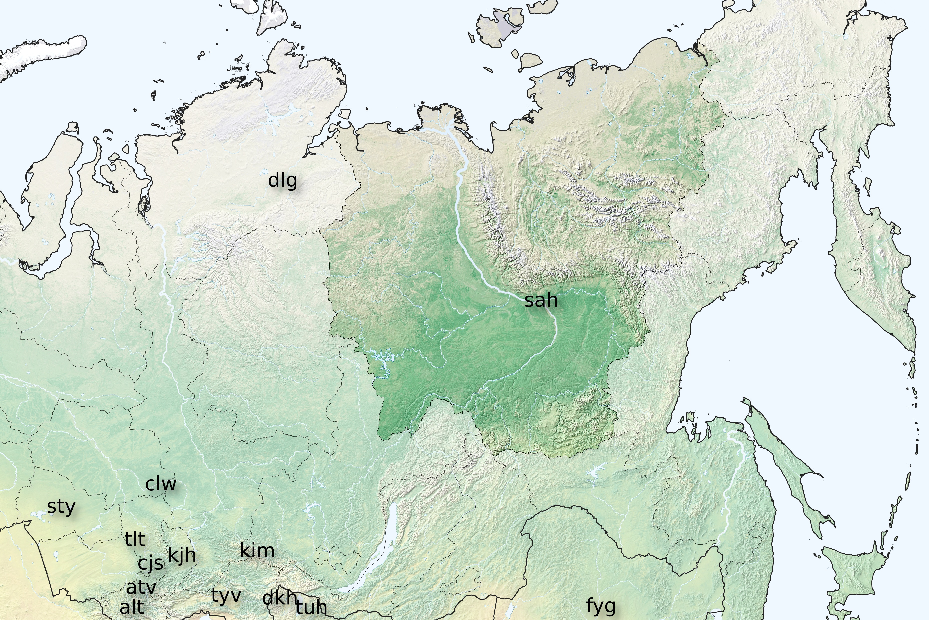
\includegraphics[width=1\textwidth]{img/map.pdf}
\end{center}

\textbf{Morphological transducers}
\begin{itemize}
\item Provide morphological \textbf{analysis} and \textbf{generation}:\\
\texttt{атын} $\leftrightarrow$ \texttt{ат\mtag{n}\mtag{px3sg}\mtag{acc}/атын\mtag{adj}/атын\mtag{post}}
\item Useful in \textbf{language technology} and \textbf{downstream tasks}:\\
spell checking, MT, CALL, text processing, etc.
\item Only one development cycle!
\end{itemize}

\section{Existing Turkic transducers}

\vspace{-0.75em}
%\begin{minipage}{0.305\textwidth}
\begin{minipage}{0.317\textwidth}
    \centering
    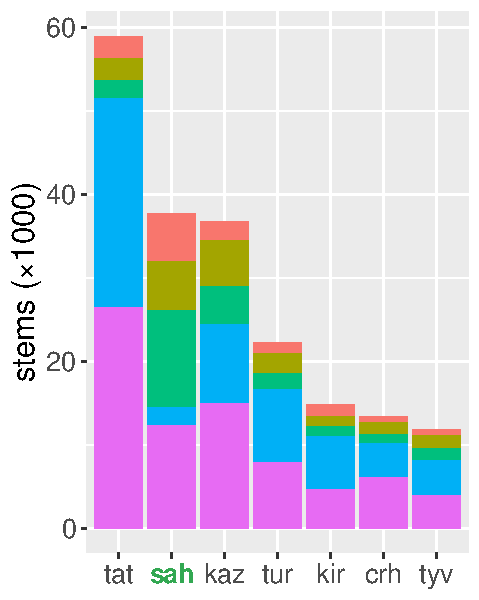
\includegraphics[width=\textwidth]{img/lgs1}\vspace{-0.8em}\\
    {\color{lightgreen}~~~~\textbf{Production}}\\
    ~~~~92\%-98\%
\end{minipage}
\begin{minipage}{0.356\textwidth}
%\begin{minipage}{0.38\textwidth}
    \centering
    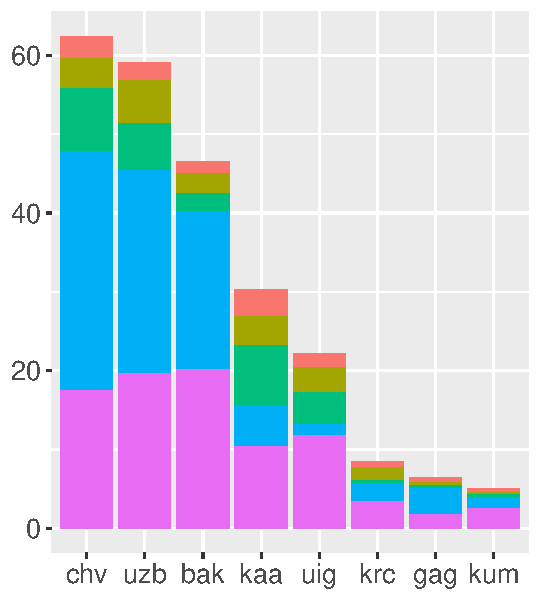
\includegraphics[width=\textwidth]{img/lgs2}\vspace{-0.8em}\\
    ~~{\color{orange}\textbf{Working}}\\
    ~~88\%-93\%
\end{minipage}
%\begin{minipage}{0.305\textwidth}
\begin{minipage}{0.317\textwidth}
    \centering
    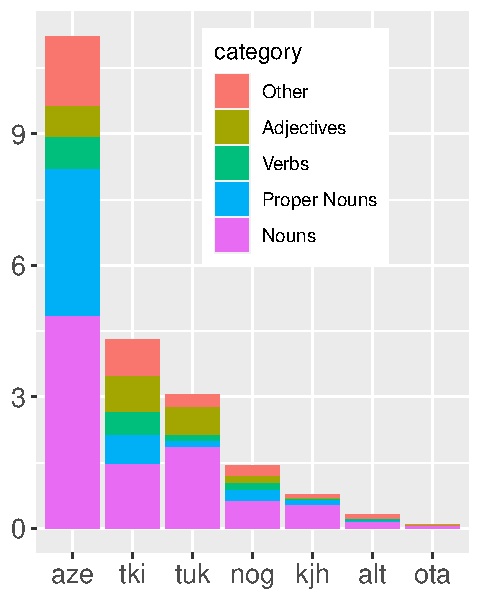
\includegraphics[width=\textwidth]{img/lgs3}\vspace{-0.8em}\\
    {\color{lightred}~~\textbf{Prototype}}\\
    ~~<80\% coverage
\end{minipage}
%\vspace{0.1pt}\hspace{2.5em}{\color{lightgreen}Production}\hfill{}{\color{orange}Working}\hfill{}{\color{lightred}Prototype}\hspace{1.5em}\vspace{0.1pt}\\

\vspace{1.5em}

%\begin{itemize}
%	\item Part of Apertium project
%	\item All 100\% free/open-source software!
%	%\item Can demo at \texttt{https://beta.apertium.org}
%\end{itemize}
\begin{center}
	({\em part of Apertium project})
\end{center}

%% This fills the space between the content and the logo
\vfill



%% Institution logo
%\includegraphics[width=\textwidth]{img/logo}\\
%
\includegraphics[height=5.5em]{img/logo-helsinki}
%
\includegraphics[height=5.5em]{img/logo-iu}
%
\includegraphics[height=5.5em]{img/logo-swarthmore}
%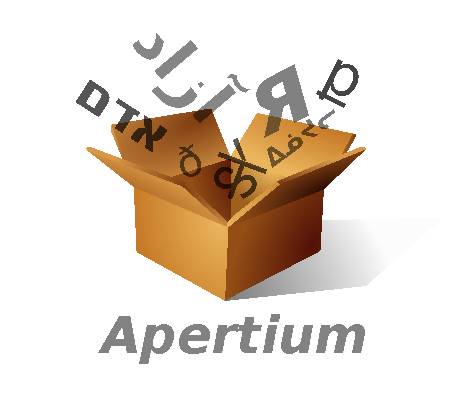
\includegraphics[height=5.5em]{img/logo-apertium}

}{
%%%%%%%% RIGHT COLUMN

\section{Implementation}
%\vspace{-1em}
\textbf{Two-level} approach using HFST, entirely \textbf{hand-coded}\\
%\begin{itemize}
    %\item entirely \textbf{hand-coded} generalisations
    %\begin{itemize}
    %    \item \textbf{\texttt{lexc}:} lexicon, morphotactics %(\texttt{lexc})
    %    \item \textbf{\texttt{twol}:} morphophonology %(\texttt{twol})
    %\end{itemize}
%\end{itemize}

%\vspace{0.25em}
%\hspace{0.5em}
%\fbox{\parbox{0.25\linewidth}{\centering
%{\setstretch{0.7}\fontsizestandard
%        Lexicon +\\Morphotactics\\}
%        \texttt{.lexc}
%}} \bigtext{\(\cap\)} % ∩
%\fbox{\parbox{0.25\linewidth}{\centering
%{\setstretch{0.7}\fontsizestandard
%        Morpho-\\phonology\\}
%        \texttt{.twol}
%}} \bigtext{=}
%\fbox{\parbox{0.3\linewidth}{\centering
%{\setstretch{0.7}\fontsizestandard
%        Morphological\\
%        transducer\\}
%        \texttt{.hfst}
%}}

\vspace{-1.5\baselineskip}
\begin{minipage}{0.7\linewidth}
\centering
\hspace{-0.1\linewidth}\orangefbox{\parbox{0.785\linewidth}{\centering
{\setstretch{0.7}\fontsizestandard
        Orthographic form\\}
        \texttt{дьиэлэрбиттэн}
}}\\\vspace{0.5em}
\bigtext{\hfill{}$\updownarrow{}$\hfill{}\}}\\\vspace{0.5em}
\hspace{-0.1\linewidth}\orangefbox{\parbox{0.785\linewidth}{\centering
{\setstretch{0.7}\fontsizestandard
        Morphological/lexical form\\}
        \texttt{дьиэ>\archi{L}\archi{A}р>\archi{B}\archi{I}>тт\archi{A}н}
}}\\\vspace{0.5em}
\bigtext{\hfill{}$\updownarrow{}$\hfill{}\}}\\\vspace{0.5em}
\hspace{-0.1\linewidth}\orangefbox{\parbox{0.785\linewidth}{\centering
{\setstretch{0.7}\fontsizestandard
        Analysis: lemma, POS, grammatical tags\\}
        \texttt{дьиэ\mtag{n}\mtag{pl}\mtag{px1sg}\mtag{abl}}
}}
\end{minipage}\qquad%\quad
%\columnbreak
\begin{minipage}{0.24\linewidth}
\vspace{3\baselineskip}
\centering
\purplefbox{\parbox{\linewidth}{\centering
{\setstretch{0.7}\fontsizestandard
        Lexicon +\\Morphotactics\\}
        \texttt{.lexc}
}}\\\vspace{0.5em}\bigtext{\(\cap\)}\\\vspace{0.5em} % ∩
\purplefbox{\parbox{\linewidth}{\centering
{\setstretch{0.7}\fontsizestandard
        Morpho-\\phonology\\}
        \texttt{.twol}
}}\\\vspace{0.75em}\bigtext{=}\\\vspace{0.75em}
\fbox{\fbox{\parbox{\linewidth}{\centering
{\setstretch{0.7}\fontsizestandard
        Morphological\\
        transducer\\}
        \texttt{.hfst}
}}}
\end{minipage}

%\begin{center}
%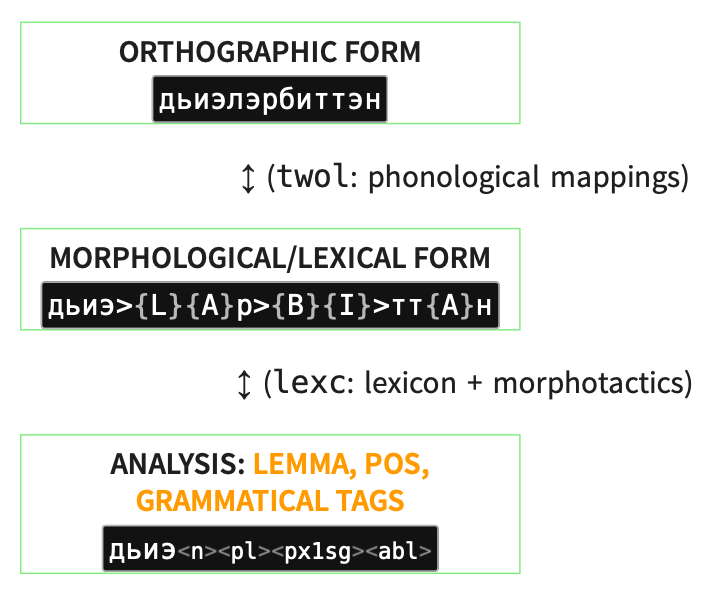
\includegraphics[width=0.7\textwidth]{img/hfst.png}
%\end{center}


\section{Evaluation: naïve coverage}

\vspace{-2em}
Number of stems that receive an analysis, correct or not\\
\vspace{-1em}

%\begin{center}
\noindent\begin{tabular}{ l r r }
 \textbf{Corpus} & \textbf{Tokens} & \textbf{Coverage} \\ 
 Newspapers & 16M & \textbf{\color{lightgreen}91.04\%}  \\
 Wikipedia & 2.4M & \textbf{\color{lightgreen}91.30\%} \\
 New Testament & 188K & \textbf{\color{lightgreen}94.53\%} \\
\end{tabular}
%\end{center}
%\vspace{0.5em}

\section{Evaluation: quality}

\vspace{-2em}
%We created a gold standard:
\begin{itemize}
\item Selected 1000 random valid wordforms from Wikipedia corpus
%\item 500 valid words of Sakha
%\item randomly selected from Wikipedia corpus
\item Manually annotated output of transducer over forms
\item \textbf{Precision:} {\color{lightgreen}\textbf{98.52\%}} (of provided analyses are correct)
\item \textbf{Recall:} {\color{orange}\textbf{75.42\%}} (of correct analyses are provided)
\end{itemize}
\vspace{-0.5em}

%\begin{description}
%    \item[Precision:] 99.9\%
%    \item[Recall:] 69.9\%
%\end{description}

%\begin{center}
%\begin{tabular}{ l r r }
% \textbf{Corpus} & \textbf{Precision} & \textbf{Recall} \\ 
% Wikipedia & 99.9\% & 69.9\% \\
%\end{tabular}
%
%\end{center}

\section{Future work}

\vspace{-2em}
\begin{itemize}
    \item Refine morphology and morphophonology
    \item Morphological and syntactic disambiguation
\end{itemize}
\vspace{-0.5em}

\section{Conclusion}

\vspace{-2em}
\begin{itemize}
    \item Robust transducer, >30k stems
    \begin{itemize}
        \item high coverage
        \item high precision (moderate recall)
        %\item moderate recall
    \end{itemize}
    %\item Ready for use in language technology applications, downstream tasks
    \item Usable in language technology applications, downstream tasks
    %\item This work has also contributed to documentation of Sakha grammar
    \item Creation contributed to documentation of Sakha grammar
    \item Free/Open Source Software (GNU GPL v3)
\end{itemize}

\vfill


\includegraphics[height=5.65em]{img/logo-helsinki}

\includegraphics[height=5.65em]{img/logo-swarthmore}

\includegraphics[height=5.65em]{img/logo-iu}
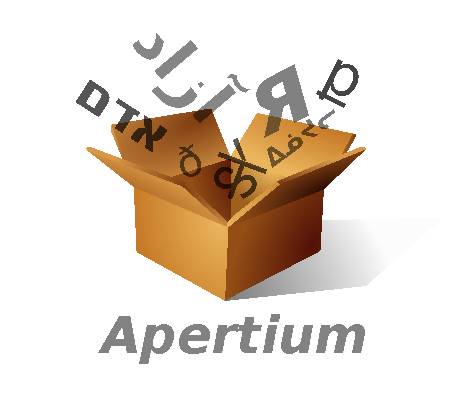
\includegraphics[height=5.65em]{img/logo-apertium}

}
\end{document}
